%--------------------------------------------------------------------------------------------------
% ips-phd-thesis-eng-ieee.tex v1.3 (see the end of the file for modification history)
% To be used with ipsthesis.cls v1.3
% 
% A template for creating a PhD thesis in English using the APA 6th edition reference formatting
% with several accompanying files.  
% By Tea Tušar <tea.tusar@ijs.si>
%
% IMPORTANT NOTE: Biber must be used as the backhand for processing bibliographies, not bibtex!
%
% To compile this template, you need to run the following sequence of commands:
% 1. pdflatex  ips-phd-thesis-eng-ieee
% 2. biber     ips-phd-thesis-eng-ieee
% 3. makeindex ips-phd-thesis-eng-ieee (optional, if you want an index)
% 4. pdflatex  ips-phd-thesis-eng-ieee 
% 5. pdflatex  ips-phd-thesis-eng-ieee
%--------------------------------------------------------------------------------------------------
\documentclass[phd,eng,ieee]{ipsthesis}
%
%--------------------------------------------------------------------------------------------------
%  
% PREAMBULE
%--------------------------------------------------------------------------------------------------
%
% Files with bibliographies 
\addbibresource{references.bib}
%
% Define here all other packages and commands you need for your thesis, for example:
\usepackage{color}
\usepackage{longtable}
\usepackage[version=4]{mhchem}

\usepackage{amssymb}
\usepackage{amsfonts}
\usepackage{amsthm}
\usepackage{amsmath}
\usepackage{mathtools}
\usepackage{subcaption}
\usepackage{comment}
\usepackage{enumitem}

\usepackage{xcolor}
\usepackage{wrapfig}
\usepackage{nicefrac}
\usepackage{floatrow}
\usepackage{siunitx}
\usepackage{epigraph} % used for chapter quotations

% for importing PDF papers (added by K. Kenda)
\usepackage{pdfpages}

% tables
\usepackage{tabu}                      % only used for the table example
\usepackage{tabularx}                      % only used for the table example
\usepackage{booktabs}                  % only used for the table example

% style lists
\usepackage{enumitem}

% algorithms
\usepackage[]{algorithm2e}
\DontPrintSemicolon

% math operators
\DeclareMathOperator*{\argmin}{arg\,min}
\DeclareMathOperator*{\cnt}{count}
\DeclareMathOperator*{\cdf}{cdf}

% Math-style definitions and theorems
% Definition
%\newtheorem{defn}[definition]{Definition} % definition numbers are dependent on theorem numbers
%\newtheorem{theorem}[theorem]{Theorem}

\newcommand{\norm}[1]{\left\lVert#1\right\rVert}

\newcommand{\error}[1]{\textcolor{red}{#1}}
\newcommand{\highlight}[1]{\colorbox{yellow}{#1}}

%\graphicspath{{figures/}}

%--------------------------------------------------------------------------------------------------
%  
% DOCUMENT
%--------------------------------------------------------------------------------------------------
\begin{document}
%--------------------------------------------------------------------------------------------------
%
% The cover page and spine are created separately using two .doc files provided by IPS.
%--------------------------------------------------------------------------------------------------
%
% FRONT MATTER
%--------------------------------------------------------------------------------------------------
%
\frontmatter
%
\selectlanguage{american}
\pagestyle{fancy}
%
% Title pages
%--------------------------------------------------------------------------------------------------
% 
% INPUT FOR THE TITLE PAGES
%--------------------------------------------------------------------------------------------------
% 
% Author
\author{Klemen Kenda}         
%
% Title in English (use \protect\\ instead of \\ to create a line break)
\titleEnglish{Pre-processing of heterogeneous data streams for Internet of Things applications}
%
% Title in Slovene (use \protect\\ instead of \\ to create a line break)
\titleSlovene{Predprocesiranje heterogenih tokov podakov za aplikacije v internetu stvari}
%
% Supervisor (title and name, affiliation)
\supervisorOne{Prof.\ Dr.\ Dunja Mladenić}{Jo\v{z}ef Stefan Institute and Jožef Stefan International Postgraduate School, Ljubljana, Slovenia}
%
% Co-supervisor (title and name, affiliation), optional
%\supervisorTwo{Dr.\ Primo\v{z} \v{S}kraba, Senior Lecturer}{Queen Mary, University of London, London, United Kingdom}
%
% Co-supervisor (title and name, affiliation), optional
%\supervisorThree{Prof.\ Name Surname3}{Institution3, Place, Country}
%
% Evaluation board chairman (title and name, affiliation)
\evaluationBoardChairman{Doc.\ Dr.\ Ale\v{s} \v{S}vigelj}{Jo\v{z}ef Stefan Institute and Jo\v{z}ef Stefan International Postgraduate School, Ljubljana, Slovenia}
%
% Evaluation board member #1 (title and name, affiliation)
\evaluationBoardMemberOne{Prof.\ Dr.\ Chrysi Laspidou}{University of Thessaly, Volos, Greece}
%
% Evaluation board member #2 (title and name, affiliation)
\evaluationBoardMemberTwo{Doc.\ Dr.\ Bla\v{z} Fortuna}{Jo\v{z}ef Stefan Institute, Ljubljana, Slovenia}
% 
% Date
\thesismonth{April}
\thesisyear{2024}
%
\maketitle 
%
% Dedication (optional)
%%--------------------------------------------------------------------------------------------------
% 
% INPUT FOR THE DEDICATION
%--------------------------------------------------------------------------------------------------
\dedication{here is no dedication now}
\makededication
%
% Acknowledgments
%--------------------------------------------------------------------------------------------------
% 
\chapter*{Acknowledgments}
\pdfbookmark[0]{Acknowledgments}{Acknowledgments}
%--------------------------------------------------------------------------------------------------

TODO
% 
% English abstract
%--------------------------------------------------------------------------------------------------
% 
\chapter*{Abstract}
\pdfbookmark[0]{Abstract}{Abstract}
%--------------------------------------------------------------------------------------------------

TODO
%
% Slovene abstract, switch to slovene
\selectlanguage{slovene}
%--------------------------------------------------------------------------------------------------
% 
\chapter*{Povzetek}
\pdfbookmark[0]{Povzetek}{Povzetek}
%--------------------------------------------------------------------------------------------------

S hitrim razvojem senzorskih tehnologij, še posebej v okviru interneta stvari (IoT), smo vstopili v obdobje, ki ga zaznamujejo velike količine podatkov, ki so na voljo v realnem času. 
S tem so nastale potrebe po novih metodah obdelave podatkov, ki omogočajo prehod od tradicionalne paketne (batch) analize do uporabe metod analize podatkov v realnem času.

Doktorska disertacija se ukvarja s prenosom analitičnih rešitev iz nadzorovanega laboratorijskega v realno okolje.
Posebej se ukvarjamo s problemi avtonomnega čiščenja, obogatitve in združevanje podatkov v realnem času, izbire značilk ter izdelave ustreznih informacijskih rešitev.
Jedro te študije predstavlja nova tehnika inkrementalnega združevanja podatkov iz heterogenih podatkovnih tokov v vektorje vektorjev značilk, primerne za uporabo v modelih strojnega učenja.
Pomembnost takšne metodologije je bila v večini študij na tem področju spregledana, saj se slednje večinoma osredotočajo zgolj na učinkovitost modelov strojnega učenja.
Te študije predpostavljajo, da so uporabljeni podatki pravilni, časovno usklajeni in vedno dostopni, kar v realnih scenarijih redko drži.

Cilj te naloge je razviti arhitekturo, ki presega zgoraj navedene privzetke. 
V disertaciji najprej predstavimo metodologijo čiščenja podatkov, ki izkorišča zmožnost Kalmanovega filtra za izdelavo kratkoročnih napovedi, vključno z napovedovanjem variance. 
Ta metoda se lahko uporablja za čiščenje podatkovnih tokov, katerih vzorčenje je veliko višje od hitrosti sprememb merjenih pojavov, kar je običajno pri internetu stvari (IoT). 
Nadalje predstavimo metodologijo za sprotno združevanje množice heterogenih virov pretočnih podatkov v vektorje značilk. 
Predlagana metodologija zmore preseči izzive, ki nastanejo zaradi heterogenih podatkovnih tokov, vključno s časovnim odstopanjem posameznih meritev in različno hitrostjo vzorčenja meritev. 
Poleg tega sistem omogoča tudi vključevanje napovedi in predhodno izračunanih vrednosti v vektorje značilk. 
S pomočjo opisane metodologije je sistem sposoben generiranja vektorjev značilk, ki vključujejo časovno usklajene podatke iz različnih virov, agregirane in obogatene vrednosti, odložene vrednosti, statične vrednosti, in vrednosti relevantnih napovedi, kot so npr. vremenske napovedi. 
Takšen sistem je sposoben ustvarjanja zelo obsežnih vektorjev značilk, ki omogočajo učinkovito modeliranje.
Velika količina značilk pa ne vodi nujno do najbolj optimalnih modelskih rezultatov, zato v nadaljevanju disertacije predstavimo še algoritem za izbiro značilk FASTENER, ki uporablja genetske algoritme in večkriterijsko optimizacijo. 
Algoritem je bil posebej zasnovan za nalogo segmentacije satelitskih slik za potrebe v kmetijstvu, vendar pa je pokazal nepričakovano učinkovitost tudi v različnih drugih primerih, npr. za napovedovanje časovnih vrst v energetiki, prometu in upravljanju z vodo. 
Vse predstavljene rešitve na koncu postavimo v lambda arhitekturo v okviru masovnih podatkov (Big Data).
Lambda arhitekturi tako dodamo analitične zmožnosti, ki niso omejene zgolj na zaznavanje dogodkov.
Predlagano arhitekturo smo uporabili pri implementaciji sistema za podporo odločanju na področju upravljanja voda. 
Na istem področju smo preizkusili tudi uporabnost algoritmov za inkrementalno učenje, kot so npr. Hoeffdingova drevesa, in jih primerjali s tradicionalnimi paketnimi metodami.

Učinkovitost predlaganega pristopa smo ocenili v več scenarijih, ki obsegajo področja, kot so upravljanje z energijo, prometom in okoljem. 
Najnovejša implementacija celotne rešitve je bila izvedena v okviru evropskega projekta H2020 NAIADES, kar dokazuje njeno uporabnost na področju upravljanja voda.
\selectlanguage{american}
%
% Contents
\maketoc
%
% List of figures (required if the thesis contains figures)
%\makelof
%
% List of tables (required if the thesis contains tables)
%\makelot
%
% List of algorithms (required if the thesis contains algorithms)
%\makeloa
%
% Abbreviations (optional)
%--------------------------------------------------------------------------------------------------
% 
\chapter{Abbreviations}
%--------------------------------------------------------------------------------------------------
%
% A command that adjusts the of vertical positioning in the abbreviations and symbols chapters
\chapteradjust
% Correct the width of columns (23pt and 377pt) to fit your needs (they should sum up to 400pt).
% Use \cr instead of \\ to break lines.
\begin{longtable}{@{}p{60pt}@{\hspace{2pt} \dots \hspace{5pt}}p{341pt}@{}}
DS & Data source \cr
FASTENER & Feature Selection Enabled by Entropy (feature selection genetic algorithm) \cr
FP7 & Seventh framework programme of the European Community for research and technological development including demonstration activities \cr 
GUI & Graphical user interface \cr
H2020 & Horizon 2020 European Union's research and innovation funding programme from 2014-2020 \cr
IoT & Internet of Things \cr
ISDI & IoT Streaming Data Integration framework \cr
LSTM & Long short-term memory \cr
ML & Machine learning \cr
MLOps & Machine learning operations \cr
SC & Scientific contribution \cr
TSDB & Time series database \cr
WMAP & Water Management Analytical Platform \cr
\end{longtable}
%
% Symbols (optional)
%%--------------------------------------------------------------------------------------------------
% 
\chapter{Symbols}
%--------------------------------------------------------------------------------------------------
%
% A command that adjusts the vertical positioning in the abbreviations and symbols chapters
\chapteradjust
% Correct the width of columns (10pt and 390pt) to fit your needs (they should sum up to 400pt).
% Use \cr instead of \\ to break lines.
\begin{longtable}{@{}p{50pt}@{\hspace{2pt} \dots \hspace{5pt}}p{390pt}@{}}
$\mathbb{R}^m$& $m$-dimensional real-valued vector space \cr
$\mathbb{R}^{+}$& positive real numbers \cr
$\mathbb{N}_m$& the first $m$ natural numbers \cr
$\norm{.}$	& norm of a vector \cr
$\left(X_n\right)_{n \ge 0}$& an infinite sequence $X_0, X_1, \dots$ \cr
$\phi$		& the embedding function \cr
$O(.)$		& the worst case asymptotic time complexity \cr
$\Theta(.)$	& the expected asymptotic time complexity \cr
$P(X)$		& the probability of event $X$ \cr
$Q$			& the transition rate matrix of a continuous time Markov chain \cr
$Q_k$		& the transition rate matrix of a continuous time Markov chain on scale $k$ \cr
$q_{ij}$	& the transition intensity between states $i$ and $j$ \cr
$q_{i}$		& the negative rate of leaving state $i$ of a Markov chain \cr
$\pi$		& the stationary distribution of a Markov chain \cr
$\Pi$		& a square matrix with the stationary distribution on the diagonal \cr
$S$			& a set of states which a Markov chain can assume (i.e. its state space) \cr
$J_k$		& a random variable which represents the times when a Markov chain switches states \cr
$H_k$		& a random variable which represents the time between two jumps of a Markov chain \cr
$c_i$		& the $i$-th centroid \cr
$C(i)$		& the Voronoi cell around the $i$-th centroid \cr
\end{longtable}
%
% Glossary (optional)
%%--------------------------------------------------------------------------------------------------
% 
\chapter{Glossary}
%--------------------------------------------------------------------------------------------------

\noindent
\emph{Time series} is a series of data points indexed in time order.

\noindent
\emph{Multivariate time series} is a time series with multiple variables.

TODO
%--------------------------------------------------------------------------------------------------
%
% MAIN MATTER
%--------------------------------------------------------------------------------------------------
%
\mainmatter
%
% Introduction
%--------------------------------------------------------------------------------------------------
% 
\chapter{Introduction}
\label{ch:introduction}
%--------------------------------------------------------------------------------------------------

\highlight{COMMENT}
V uvodu magistrskega dela oz. doktorske disertacije mora biti jasno povzeta teza iz prijave teme magistrskega dela oz. doktorske disertacije. Dosežki so praviloma predstavljeni strokovni javnosti. Glavno besedilo magistrskega dela oz. doktorske disertacije se lahko nadomesti z objavami (oziroma z deli, sprejetimi v objavo) v uglednih mednarodnih revijah.

To pomeni, da praviloma poglavja v disertaciji ostanejo enaka, le da namesto poglavij, v katerih bi praviloma dokazovali posamezno hipotezo, zamenjate s članki (1 članek = 1 poglavje), v uvodu posameznega poglavja s člankoma pa navedete opis znanstvene metode ter vaš prispevek k posamezni objavi.
\highlight{ENDCOMMENT}

\section{Motivation}
\highlight{Motivacija / goals}

\section{Scientific Contributions}
\highlight{aims and hypothesis / contributions to science}

\section{Architecture}

\highlight{THE BIG PICTURE}

The document is structured as follows: \highlight{TODO}
%--------------------------------------------------------------------------------------------------
% 
\chapter{Autonomous Data Cleaning on a Stream}
\label{ch:data-cleaning}
%--------------------------------------------------------------------------------------------------

\highlight{COMMENT}
V tem primeru mora biti iz uvoda jasno razviden opis znanstvene metode ter prispevka kandidata k posamezni objavi, pri kateri je več avtorjev. V diskusiji kandidat smiselno povzame vse rezultate svoje disertacije.
\highlight{ENDCOMMENT}

TODO

\begin{list}{}
{\leftmargin=2.5em \itemindent=-2.5em}
    \item K. Kenda and D. Mladenić, “Autonomous sensor data cleaning in stream mining setting,” \textit{Business Systems Research Journal}, vol. 9, no. 2, pp. 69–79, 2018.
\end{list}


\begin{quote}
    \textit{Klemen Kenda contributed to the conceptualization, methodology, software development, evaluation and visualization. He also lead writing of the paper.}
\end{quote}

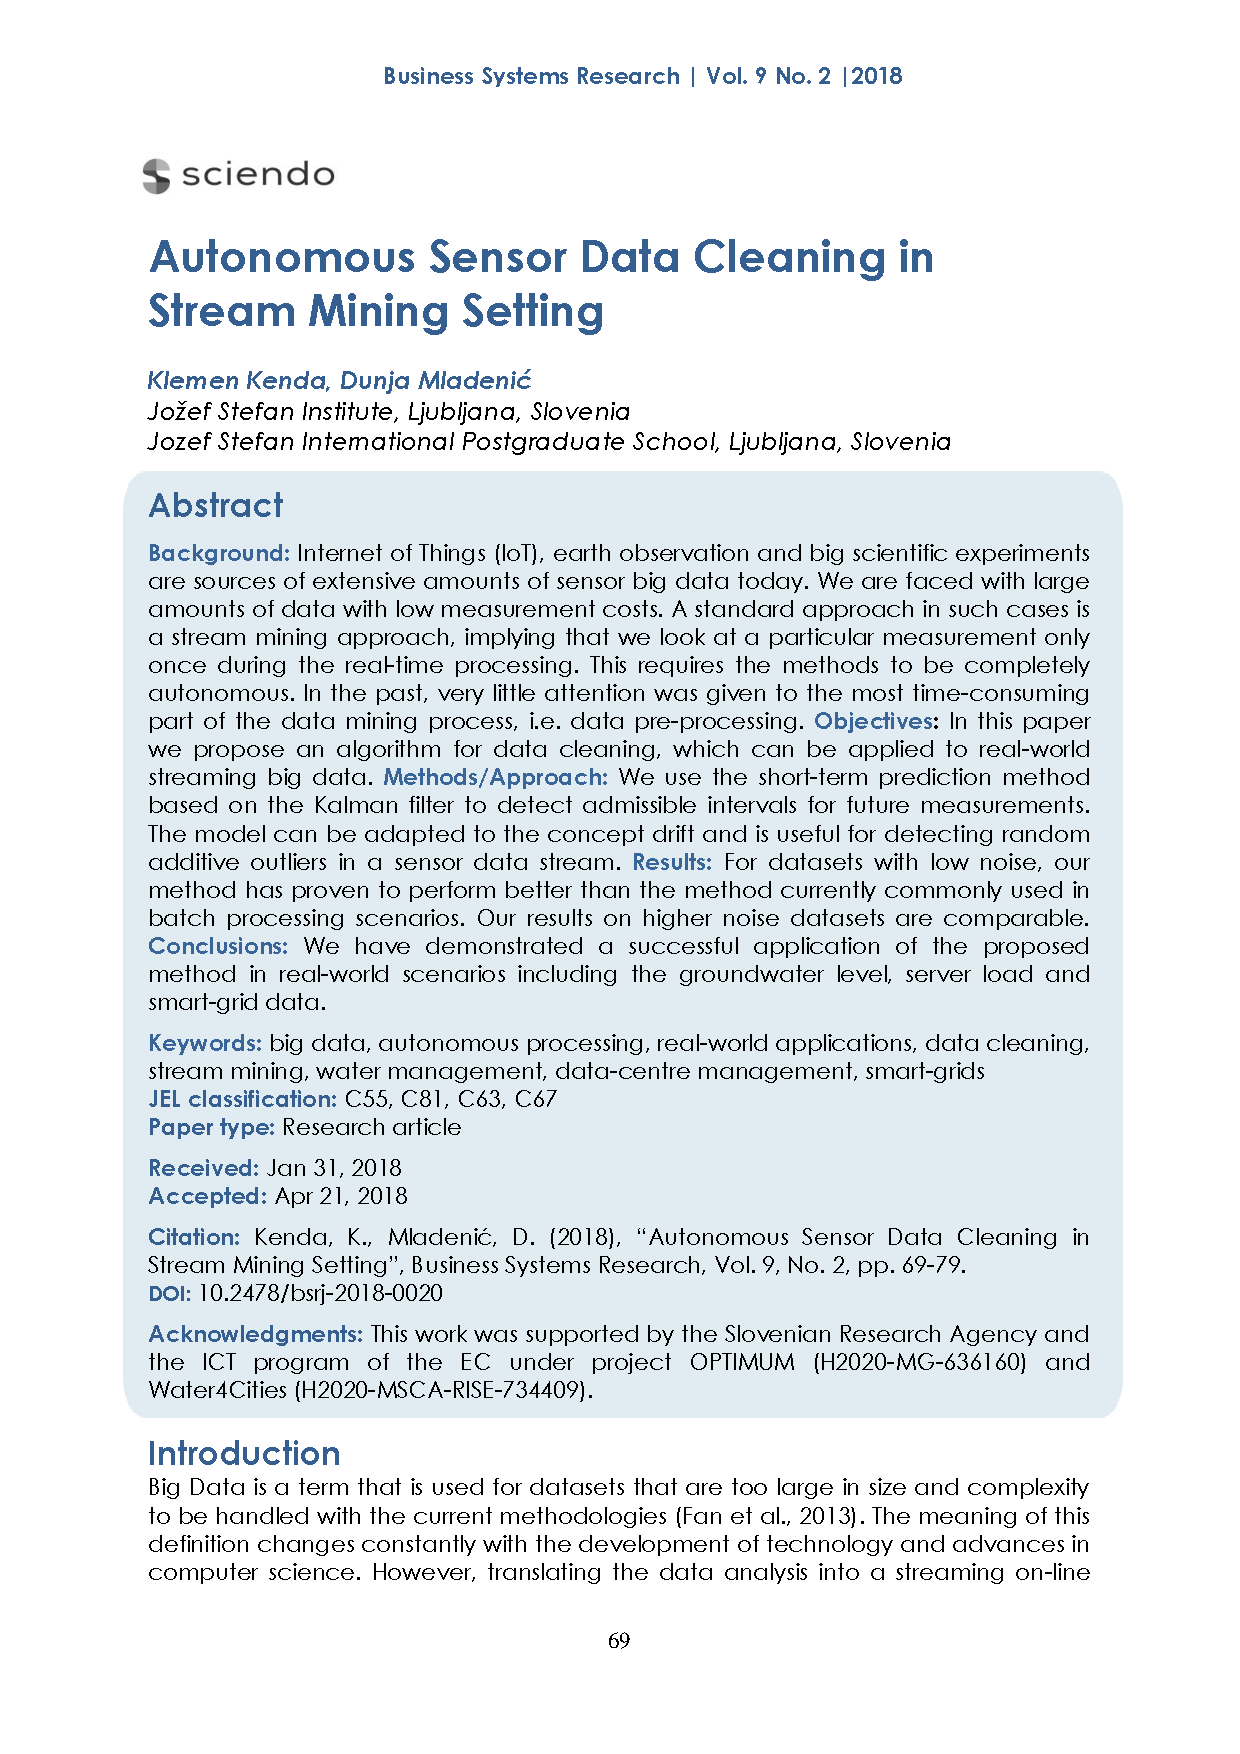
\includepdf[pages=-]{papers/data_cleaning.pdf}
%--------------------------------------------------------------------------------------------------
\chapter{Heterogeneous Streaming Sources Data Fusion for Machine Learning}
\label{ch:data-fusion}
%--------------------------------------------------------------------------------------------------

\epigraph{Data fusion is like a marriage: integrating data sources together requires patience, compromise, and a common language.}{\textit{Kirk Borne}}

% anouncing the paper
\begin{quote}
This chapter presents the paper titled \textit{Streaming data fusion for the internet of things} by Klemen Kenda, Blaž Kažič, Erik Novak and Dunja Mladenić and presents the centerpiece of this thesis. The paper was published in the Sensors journal \cite{kenda:2019:fusion}.
Klemen Kenda is the main author of the paper. 
He contributed to conceptualization, methodology, software development, validation, formal analysis, data curation, writing, visualization, project administration and funding acquisition.
\end{quote}

% introduction
In the context of the Internet of Things (IoT), data fusion, also known as sensor data fusion or information fusion, refers to the process of combining and integrating data from multiple sensors or sources to create a more accurate, comprehensive, and meaningful representation of the environment or system being monitored. 

The main goal of data fusion in IoT is to extract valuable insights, improve decision-making, and enhance the overall efficiency of IoT applications. 
By fusing data from multiple sensors, the resulting information can provide a more accurate understanding of the environment, which can result in better modeling capabilities such as creating predictions or anomaly detection, and a more holistic view of the system's behavior. 

%\highlight{Role of semantic fusion?}
There are several types of data fusion techniques used in IoT, that vary from local to more global approaches and are based on the JDL model \cite{hall:2001:multisensor}:
\begin{enumerate}
    \item \textbf{Sensor-level Fusion:} This involves combining raw sensor data at the individual sensor level to reduce noise and errors. It can include techniques like filtering, calibration, and data alignment.
    
    \item \textbf{Feature-level Fusion:} In this approach, extracted features from the data of different sensors are combined to create a more informative representation. This can help in reducing data dimensionality and improving the efficiency of analysis.
    
    \item \textbf{Decision-level Fusion:} Here, the outputs or decisions from multiple sensors are combined to make a more reliable decision. This technique is often used to improve accuracy and robustness in applications like object tracking or localization.
    
    \item \textbf{Information-level Fusion:} This is the highest level of fusion, where higher-level knowledge or context is integrated into the data to create a comprehensive understanding of the situation. This can involve incorporating external data sources, historical data, or expert knowledge.
\end{enumerate}

% introduction to paper
Our methodology focuses on feature-level fusion and is ignorant of any high-level semantic information regarding the observed system, such as sensor metadata or even system's knowledge graph \cite{kenda:2019:fusion}. 
The goal of the research was to create a useful component in the lambda architecture that would enable fast deployment of real-world IoT applications of machine learning, such as predictive modeling or anomaly detection.

% methodology
The paper provides a formal definition of heterogeneous data streams fusion, a working streaming data fusion framework and conceptual architecture of the system.
In the lambda architecture, the data fusion component is located immediately after data cleaning (see Figure \ref{fig:the_big_picture}).

The methodology is able to ingest 3 types of data: streaming sensor data, updating predictions (such as weather forecasts) and static data (such as data describing human behaviour, for example working days).
Three algorithms are presented that enable the framework to generate enriched data streams and fuse them locally and globally.

% evaluation
The system has been deployed both in a cloud environment and on an edge device. 
Validation of the methodology's efficiency has been accomplished through cloud deployment, using public train data from edge devices on the smart-grid dataset. Additionally, performance evaluation was conducted on the traffic dataset.

The findings strongly support the advantages of employing data fusion techniques. Enhanced data streams have demonstrated a higher model accuracy when compared to non-enriched streams. Moreover, the utilization of multiple data streams that provide contextual information has yielded superior model outcomes in comparison to relying solely on single-source data streams.

The implemented system has been successfully deployed across two distinct environments: a cloud-based infrastructure and an edge computing device.
In a cloud-based deployment, the methodology's efficiency has been validated on the smart-grid dataset. 
On the edge devices, deployed in electric public trains, the methodology's effectiveness has been validated on the traffic dataset.

The results confirm the benefits of using data fusion methods: enriched data streams yield better model accuracy than non-enriched and streams from multiple data streams that describe more context yield better model results than single source data streams.
Additional validation of the overall system water management scenarios is given also in Chapter \ref{ch:big_data_framework}.

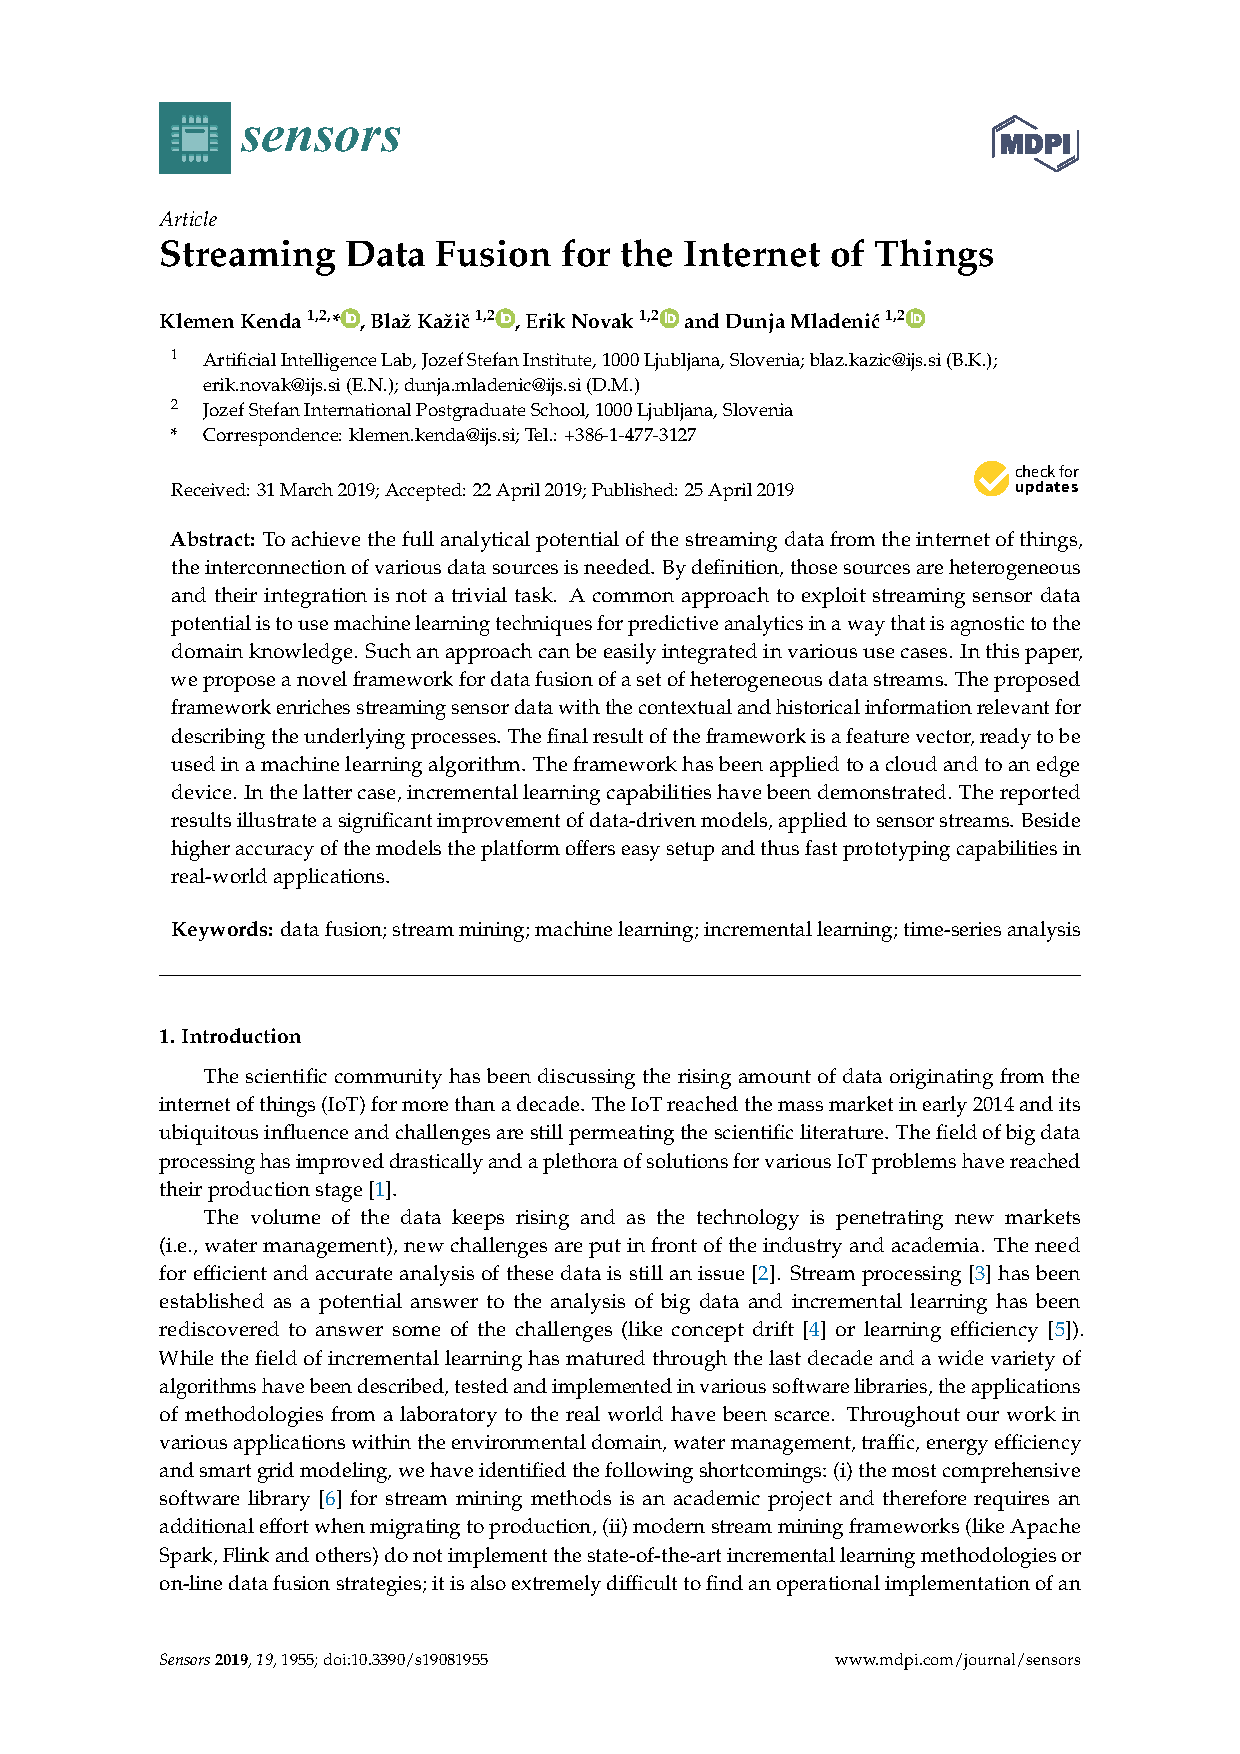
\includepdf[pages=-]{papers/streaming_data_fusion_for_iot.pdf}
%--------------------------------------------------------------------------------------------------
% 
\chapter{Feature Selection using Multi-Objective Optimization}
\label{ch:feature-selection}
%--------------------------------------------------------------------------------------------------

TODO

\begin{list}{}
{\leftmargin=2.5em \itemindent=-2.5em}
    \item F. Koprivec, K. Kenda, and B. Šircelj, “FASTENER feature selection for inference fromearth observation data,” \textit{Entropy}, vol. 22, no. 11, p. 1198, 2020.
\end{list}

\begin{quote}
    \textit{Klemen Kenda and Filip Koprivec share the first autorship of the paper.
    Klemen Kenda contributed to conceptualization and methodology, validation, writing and also to project administration and funding acquisition. 
    Klemen Kenda was supervising the work of the other co-authors.}
\end{quote}

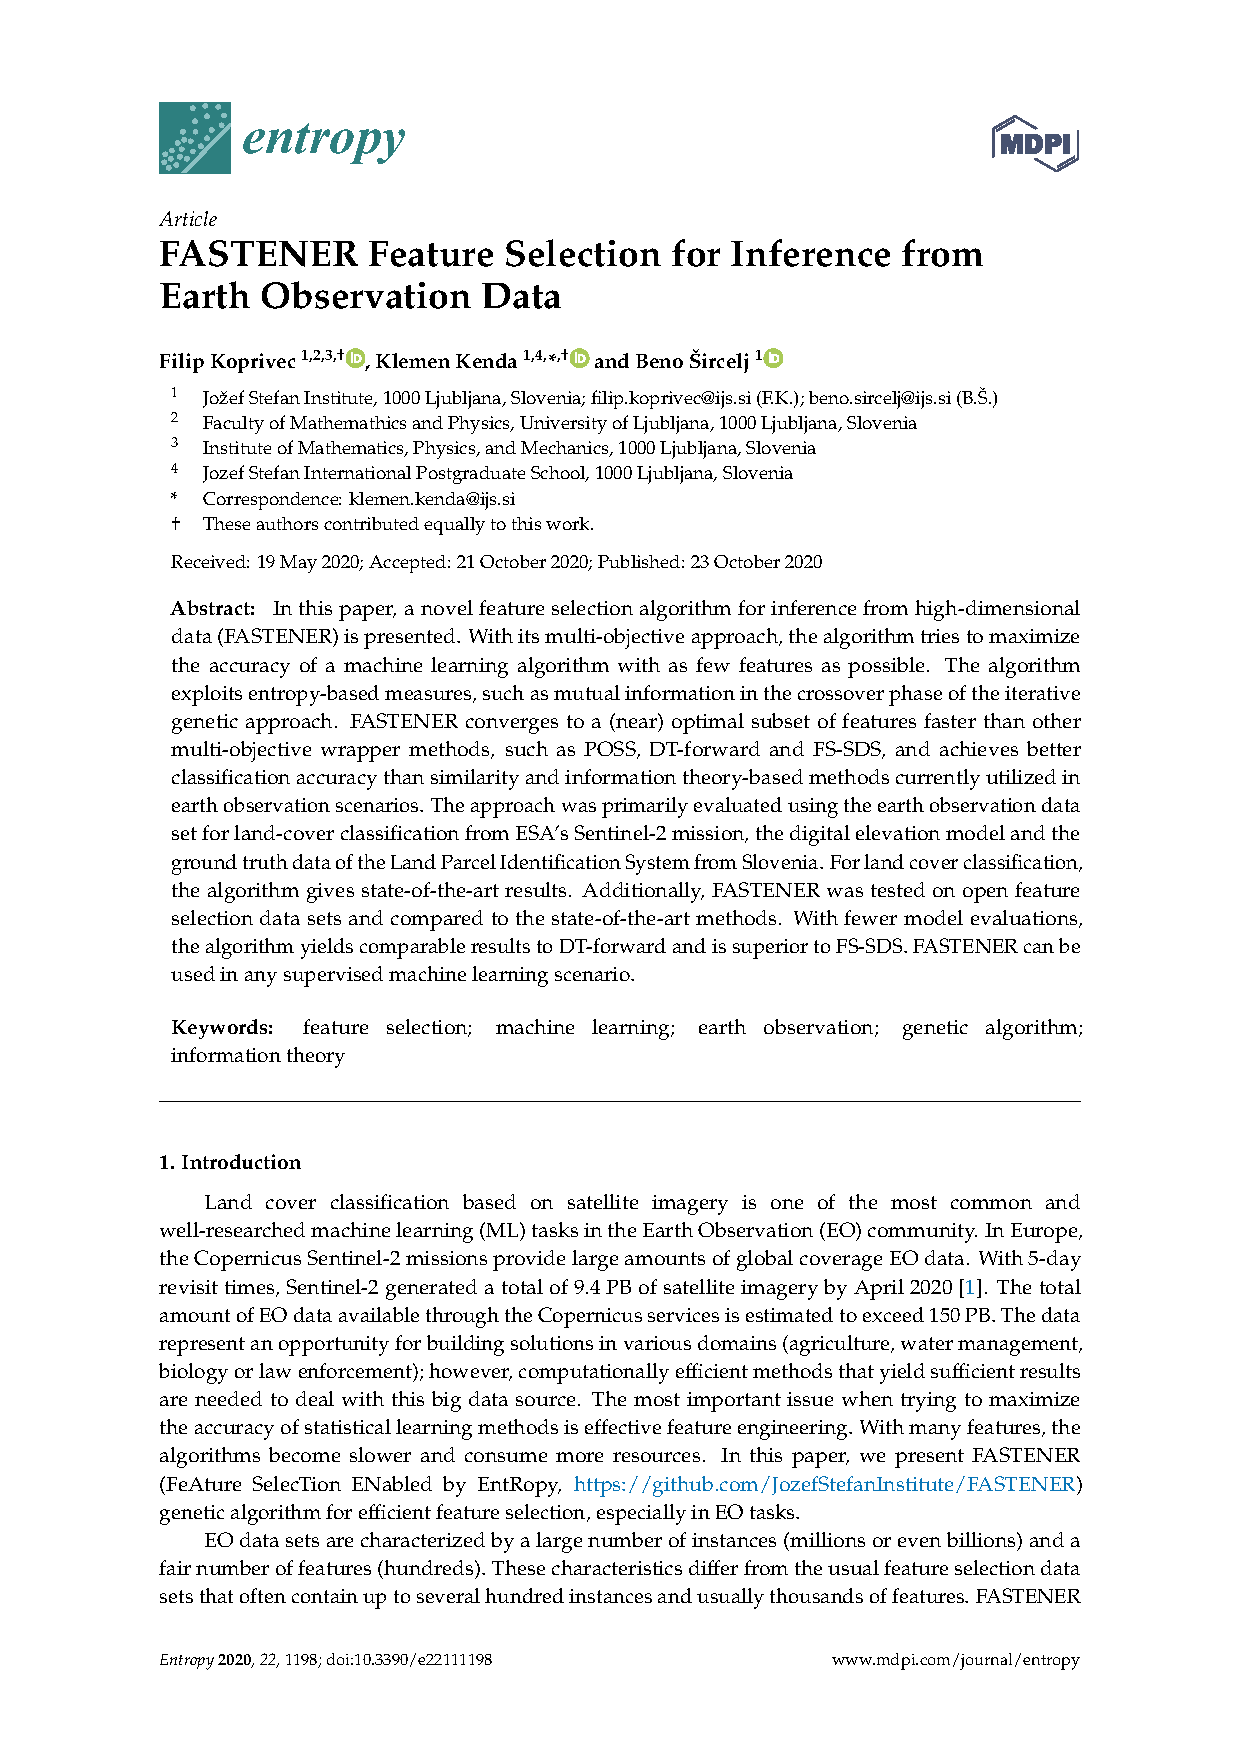
\includepdf[pages=-]{papers/fastener.pdf}




%--------------------------------------------------------------------------------------------------
% 
\chapter{Big Data Framework for Water Management}
\label{ch:results}
%--------------------------------------------------------------------------------------------------

\section{Framework}
\highlight{TODO}

\section{Evaluation}
\highlight{TODO}


\begin{list}{}
{\leftmargin=2.5em \itemindent=-2.5em}
    \item K. Kenda, J. Peternelj, N. Mellios, D. Kofinas, M. Čerin, and J. Rožanec, “Usage of sta-tistical modeling techniques in surface and groundwater level prediction,” \textit{Journal ofWater Supply: Research and Technology—AQUA}, vol. 69, no. 3, pp. 248–265, 2020.
\end{list}

\begin{quote}
    \textit{Klemen Kenda contributed significantly to conceptualization and methodology development presented in this paper. 
    He contributed to software development, design and implementation of evaluation.
    He lead the writing of the paper and also contributed to visualizations.}
\end{quote}

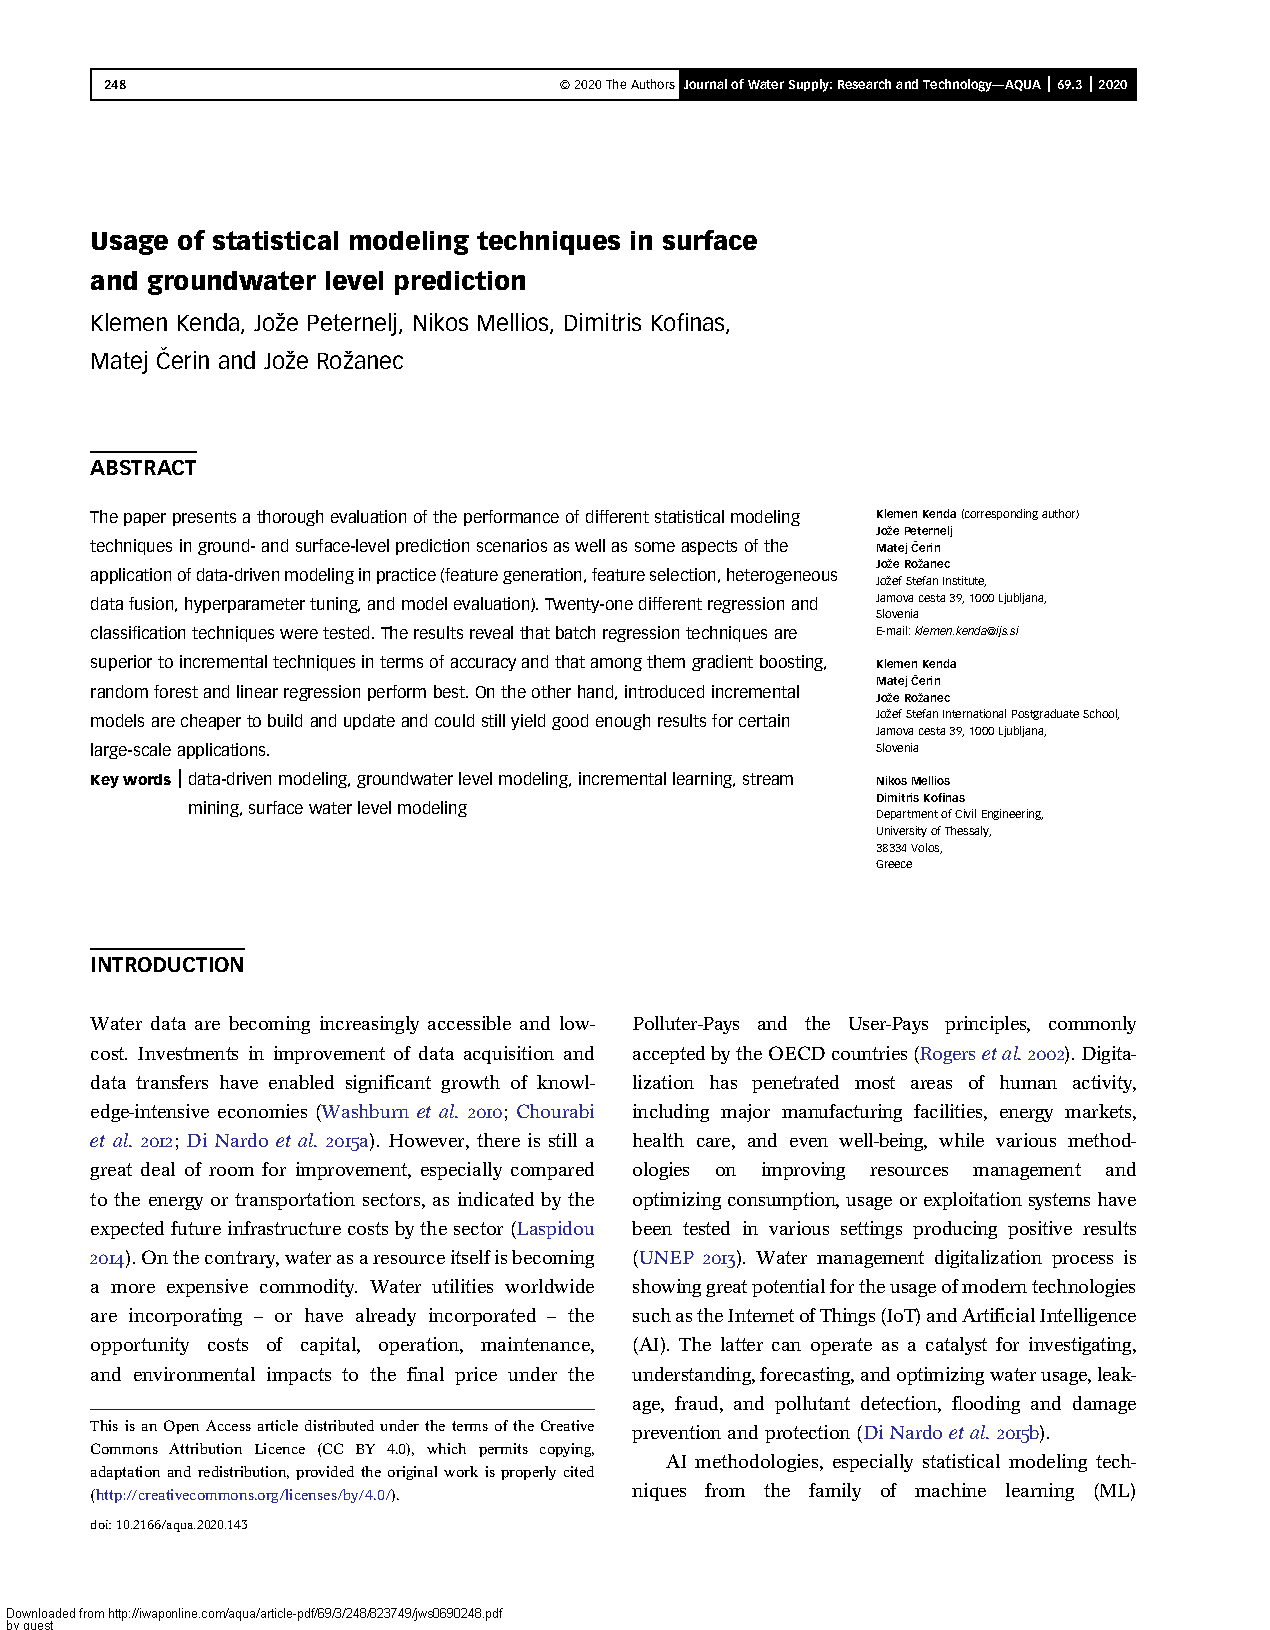
\includepdf[pages=-]{papers/water_level_prediction.pdf}
%--------------------------------------------------------------------------------------------------
% 
\chapter{Conclusions and Further Work}
\label{ch:conclusion}
%--------------------------------------------------------------------------------------------------

\epigraph{The only thing that makes life possible is permanent, intolerable uncertainty; not knowing what comes next.}{\textit{Ursula K. Le Guin}}

This thesis investigates the entire vertical needed to handle multiple heterogeneous time series analysis and the implementation of predictive models for IoT in real-world scenarios.
The contributions are significant in terms of the architectures and frameworks involved, as well as the development of data cleaning and pre-processing capabilities, and ultimately modeling. 
The focal point of the thesis is the framework for autonomous online fusion of heterogeneous sensor streams data, which serves as the foundation for many other features of the proposed platform, including efficient modeling with contextual data and real-time prediction generation.

We have proposed several new algorithms and innovations.
A new algorithm using Kalman filtering has been suggested for autonomous online time series data cleaning. 
A new approach for online data fusion of heterogeneous data streams in predictive modeling has been introduced. 
A feature selection algorithm, called FASTENER, has been proposed, which utilizes genetic algorithms and multi-objective optimization methods to achieve faster convergence and improved feature sets compared to previous methods.
To the best of our knowledge, the usability of incremental learning methods in water management scenarios has been analyzed for the first time. 
Lastly, an extension to the Big Data lambda architecture has been proposed, enhancing the predictive capabilities of the analytical frameworks in the speed (online) pillar.

The solutions described in this thesis have been developed and validated as part of our activities in several research projects funded by the FP7 and H2020 programs and have also been implemented in industry. 
The entire range of applications has been utilized and deployed in the H2020 NAIADES project, where it was enhanced with various specific water management solutions. 
The thesis encompasses numerous evaluations conducted in the fields of environment, transportation, energy, and Earth observation.

In the rest of this chapter, we begin by providing a summary of the scientific contributions made in this thesis. 
We then proceed to discuss the goals and hypotheses presented in Chapter \ref{ch:introduction}, taking into account our contributions and results. 
Finally, we conclude by outlining some potential directions for future research.

\section{Contributions to Science}
\label{sec:contributions_to_science}

%Še enkrat se prispevke zananosti napiše in razdela; kako smo te stvari dokazali (lahko številke iz rezultatov).

\noindent The scientific contributions of the thesis lie in the domains of data pre-processing, big data architectures. 
We also offer an assessment of the developed methodologies in various real-world scenarios.
Below, we will further divide each contribution and provide a brief discussion and evaluation for each.\\

\noindent \noindent \textbf{SC1 - Novel methodologies for data cleaning, data fusion and feature selection}: 
%Development of autonomous methodologies for online data cleaning (based on Kalman filter), fusion and enrichment of heterogeneous data streams. Development of a novel algorithm for feature selection based on information theory and multi objective optimization approach.
\begin{itemize}
    \item \textbf{SC1.1 - Incremental data cleaning}: 
        We have developed an incremental data cleaning methodology based on Kalman filter.
        Our approach demonstrates that this methodology can be initialized without prior knowledge regarding the data stream to be cleaned, making it well-suited for application in IoT data streams, where periodicity of the observed phenomena is typically considerably shorter than the sampling interval.
        To evaluate our methodology, we conducted tests on a variety of datasets, including one synthetic labeled dataset and six unlabeled datasets, consisting of two synthetic datasets and four real-world datasets.
        Within the unlabelled datasets, we have implemented an outlier detection assessment based on the outcomes of autoregressive modeling. The results clearly indicate that the cleansed datasets lead to improved modeling results.
    \item \textbf{SC1.2 - Incremental data enrichment and data fusion:} 
        We have introduced a formal definition of heterogeneous data streams fusion. 
        In this formal definition, we establish the essential components, encompassing data streams and the requisite operators, which collectively yield the generation of enriched feature vectors that enable more accurate predictive modeling.
        We developed a generic streaming data fusion framework for heterogeneous data streams. 
        To the best of our knowledge, we provided the first generic framework capable of generating feature vectors from heterogeneous data streams, thereby enabling the application of machine learning techniques in real-time streaming scenarios.
        We demonstrated the usability of the platform beyond the controlled laboratory environment, integrating it in several real-world pilot scenarios.        
    \item \textbf{SC1.3 - Feature selection:}
        We proposed a novel genetic wrapper algorithm for feature selection that we coined FASTENER (feature selection enabled by entropy).
        The algorithm reduces the number of features in a machine learning problem while preserving or even improving modeling accuracy.
        Using pre-trained models for information gain calculation, the algorithm converges faster towards the optimal feature set for a particular modeling task than similar algorithms.
        The algorithm improved state-of-the-art accuracy in the remote sensing application for land-cover classification and has also shown competitive performance on several feature selection benchmark datasets (with very small samples and very big number of features).        
\end{itemize}

\noindent \textbf{SC2 - Extension of lambda architecture}: 
%Development of an extension of lambda (big data) architecture for hybrid ML model development (batch) and deployment (in real-time).
\begin{itemize}
    \item \textbf{SC2.1 - Extended lambda architecture:}
        The proposed analytical platform is based on the lambda and hut architectures.
        We suggested refinements of the big data architectures in order to support the needs in the water domain.
        In the lambda architecture, we suggested to include modeling capabilities in the speed pillar to overcome the traditional capabilities, limited to (complex) event processing.
    \item \textbf{SC2.2 - Conceptual architecture for water management analytical platform based on extended lambda architecture:}
        A solution for heterogeneous sources data fusion in a stream was integrated in the architecture.
        The setting enables contextual information to be included in the data-driven models.
        This contribution enables integration of machine learning applications to the real world scenarios and overcomes the laboratory setting for testing of forecasting or anomaly detection models on a stream of data.
        
\end{itemize}

\noindent \textbf{SC3 - Evaluation in real-world scenarios}: 
%Evaluation of the proposed architecture and methods in several real-world scenarios from the energy management, water management, smart cities, transport energy management and earth observation domains.
\begin{itemize}
    \item \textbf{SC3.1 - Evaluation of the proposed architecture and methods in several real-world scenarios: }
        We successfully integrated a solution for heterogeneous sources data fusion in a stream in the architecture.
        Such a setting not only facilitates the inclusion of contextual information in data-driven models but also culminates in a notable enhancement of the overall model accuracy.

        The initial ideas for this work have been developed already in 2014 within FP7 NRG4CAST project and then later implemented also in FP7 Sunseed project, where data fusion has been utilized in the energy management sector, handling forecasting of energy demand/production in thermal plants, smart buildings, smart cities and smart grids.
        The implementation of smart grid solutions was successfully executed within the project in collaboration with Iskratel d.d. Furthermore, these solutions were effectively deployed in their commercial applications.
        Further development followed during the H2020 In2Dreams project, where the infrastructure has been used in the mobility use case, mainly estimating energy consumption of electric trains for short- and mid-term prediction horizons.
        The usability of data fusion has been studied for land-cover applications based on satellite imagery in H2020 PerceptiveSentinel project, where FASTENER feature selection has been developed.
        Finally, the lambda framework has been formalized in H2020 Water4Cities and H2020 NAIADES projects. 
        The former provided a rich implementation of the framework (including data fusion, anomaly detection, predictions and complex domain applications) in the water management sector.
        
        The papers presented in this thesis also include evaluation of presented methodologies with the focus on the benefits of heterogeneous on-line sensor data fusion in several scenarios: environmental scenarios \cite{kenda:2018:autonomous, kenda:2020:water-modeling, kenda:2022:water-framework}, energy management~\cite{kenda:2019:fusion}, transport~\cite{kenda:2019:fusion}, and Earth observation~\cite{koprivec:2020:fastener}.
    \item \textbf{SC3.2 - Evaluation of incremental learning methods in the water domain: }
        Stream mining techniques improve the computational performance of the pipeline and provide models that are better able to adjust to changes (concept drift) in real-time data than traditional batch models.
        The architecture natively supports incremental methods, covered in SC1, and therefore fits well with incremental learning techniques.
        We introduced incremental learning techniques to modeling of surface and groundwater levels.
        In that scenario, we prepared a comparison of 21 different statistical modeling techniques at different time horizons.    
\end{itemize}

\section{Further Work}

The thesis proposes solutions for applications of anayitics in IoT, addressing a broad variety of challenges through the entire data processing vertical, specifically in data cleaning, data fusion, feature selection, predictive modeling, and the corresponding architectural design. 
In the further work section, we limit ourselves to the areas where this thesis provides the most significant contributions.
Further work is outlined in three categories: applications, architecture and data fusion. 
In the latter part, we also acknowledge and discuss the significant influence of deep learning models on the accomplishments presented in this thesis. \\

% other domains
\noindent \textbf{Applications.} 
One potential avenue for further research would involve assessing the performance of the proposed system in various other contexts, such as smart cities, smart buildings, smart agriculture, health care, finance, manufacturing, and other relevant domains.
The unique characteristics of different domains may provide valuable insights to enhance the functionality of the presented components to better meet the specific requirements of use cases. \\

% architecture
\noindent \textbf{Architecture.} 
From an architectural perspective, there are a couple of potential directions to consider. 
An intriguing enhancement to the current system could be the implementation of a feature store, which would extend the current data management layer. 
As feature vectors are generated in an incremental manner, the feature store would greatly enhance the system's usability and also offer improved traceability and troubleshooting capabilities for data engineers.

The need to automate and operationalize machine learning models has led to a new field within computer engineering and data science called machine learning operations (MLOps)~\cite{kreuzberger:2023:mlops}.
Several new architectures have been proposed in the field in recent years that present end-to-end ML frameworks, which address and solve similar problems as enhanced lambda architecture.
The solutions rely on horizontally scalable elements capable of managing large volumes of data from the Internet of Things (IoT) and other sources.
Future research should take into account the potential impact of recent achievements in MLOps to the rationality and efficacy of the proposed lambda architecture.
\\

% data fusion
\noindent \textbf{Data fusion.}
The limitations of the custom data fusion components have been observed through practical experience. 
These include issues such as the delayed calculation of features that rely on a significant amount of historical data for computation, as well as the complex process of restarting the system after a crash or the injection of invalid data.
The latter situation often occurs during the development of a new model and, therefore, represents a bottleneck in the whole modeling cycle.
Over the past few years, there has been a significant increase in the popularity of time series databases (TSDB), leading to the development and availability of several mature implementations.
Utilizing the capabilities of TSDB's, a data fusion approach would conceptually represent a regression from the presented incremental data fusion algorithms. 
Nevertheless, the anticipated outcome would offer improved stability and faster prototyping of machine learning solutions.

Evaluation of data fusion systems is difficult and is usually achieved through its effect on modeling capabilities.
We propose a future investigation of the evaluation of the level of expressiveness of the language used to define feature vectors.

The connection between the data fusion component and its applicability in time series deep learning models has not been explored in our research.
By utilizing Long Short-Term Memory (LSTM), the models have acquired the capability to retain information in memory over extended periods of time.
Models like these have shown great success in processing sequential data, such as in analyzing time series.
The ability to recall information may make certain aspects of the data fusion component obsolete, such as including delayed measurements in the feature vector.
A similar effect could be achieved with self-attention mechanisms in transformers and other relevant deep learning approaches (N-BEATS~\cite{oreshkin:2019:nbeats}, N-HiTS~\cite{challu:2023:nhits}, PatchTST~\cite{nie:2022:time}).
Additional studies are needed to determine the extent to which data fusion contributes to the performance of deep neural network models.

Driven by the success of ChatGPT and other large language models, several proposals have emerged recently for foundational models for time series.
One such example is TimeGPT-1 \cite{garza:2023:timegpt}, which is very successful with zero-shot inference of volatile time series.
In the coming years, significant advancements are expected with these types of models, which could potentially provide a feasible alternative to current time-series modeling approaches.
Because multivariate time series are not considered in these models, our approach may consistently outperform foundational time-series models for several use cases from presented domains.
We recommend that future research examines the usability of foundational models for time series in use cases that involve relevant contextual data.



%--------------------------------------------------------------------------------------------------
%
% APPENDICES (optional)
%--------------------------------------------------------------------------------------------------
%
%\appendix
%\begin{appendices}
%
% For example, proofs of theorems could be an appendix
%%--------------------------------------------------------------------------------------------------
% 
\chapter{Configuration and Parameters}
\label{app:parameters}
%--------------------------------------------------------------------------------------------------

TODO

\section{Dataset and Attribute Selection}

TODO

\section{Attribute Configuration}

TODO
%
%\end{appendices}
%--------------------------------------------------------------------------------------------------
%
% BACK MATTER
%--------------------------------------------------------------------------------------------------
%
\backmatter
%
% References used in the thesis
\printreferences
% 
% Author's bibliography 
%--------------------------------------------------------------------------------------------------
% 
\chapter{Bibliography}
%--------------------------------------------------------------------------------------------------
% Enclose with refsection and use \nocite{*}, if you need to list publications not referenced in 
% the thesis:
\begin{refsection}
\nocite{*}

\section*{Publications Related to the Thesis}

\noindent

\defbibheading{subbibliography}{\subsection*{Journal Articles}}
\printbibliography[heading=subbibliography,env=nolabelbib,keyword=myarticle]

\defbibheading{subbibliography}{\subsection*{Conference Papers}}
\printbibliography[heading=subbibliography,env=nolabelbib,keyword=myconf]


\section*{Other Publications}

\noindent

\defbibheading{subbibliography}{\subsection*{Journal Articles}}
\printbibliography[heading=subbibliography,env=nolabelbib,keyword=myotherarticle]

\defbibheading{subbibliography}{\subsection*{Book Chapters}}
\printbibliography[heading=subbibliography,env=nolabelbib,keyword=mybook]

\defbibheading{subbibliography}{\subsection*{Conference Papers}}
\printbibliography[heading=subbibliography,env=nolabelbib,keyword=myotherconf]

\end{refsection}
%
% Author's biography
%--------------------------------------------------------------------------------------------------
% 
\chapter{Biography}
%--------------------------------------------------------------------------------------------------

\begin{wrapfigure}{o}{0.25\textwidth}
    \vspace{-0.5cm}
    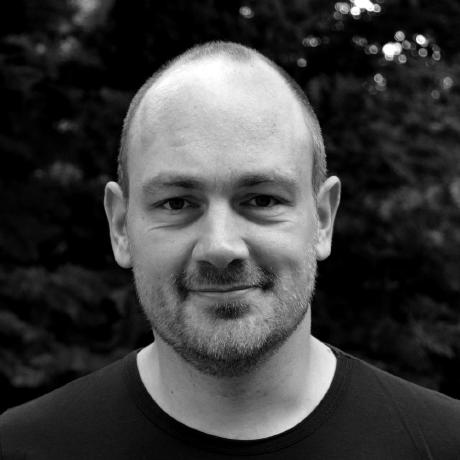
\includegraphics[width=1\linewidth]{figures/klemen_kenda_qlector.jpg} 
    \label{fig:portrait}
\end{wrapfigure}

Klemen Kenda is a researcher at Jozef Stefan Institute and Qlector d.o.o.
He obtained his diploma in physics at University of Ljubljana and is pursuing his PhD in Information and Communication Technologies at Jožef Stefan International Postgraduate School. 

His broad early working experience include development of control systems for large physics experiments at Sinchrotrone Trieste and Forschungzentrum Karlsruhe (collaboration with F2 department at JSI, later Cosylab), data analysis for online advertising at Httpool d.o.o., implementing geospacial solutions at DFG Consulting, analysing environmental software at Environmental agency of Slovenia, independent web development, teaching of physics, mathematics and programming at Primary school Cerkno and Gimnazija Jurija Vege Idrija, managing public relations at Scout association of Slovenia and several local, national and international management positions within Slovenian orienteering federation.

As a researcher, he has been involved with machine learning and stream mining of heterogeneous data sources. 
Applications of his work have been made in the fields of environmental intelligence, production planning and energy management. 
From 2011, he has contributed to several EU FP7, H2020 and Horizon Europe projects (Planetdata, Envision, NRG4CAST, Sunseed, PerceptiveSentinel, EnviroLENS, Factlog, Water4Cities, NAIADES, STAR, AquaSPICE, APRIORI, Plooto and HumAIne) and acted as a leader of several technical tasks and work packages. 

As a researcher, he has been involved in the Qlector company, firstly as QlectorLEAP developer and later as EU project leader.
Beside being used in several EU projects, his work described in the thesis has been implemented in several use cases also in industry. 
%Iskratel d.o.o.
%
% Index (optional)
% \printmyindex
%--------------------------------------------------------------------------------------------------
\end{document}
%--------------------------------------------------------------------------------------------------
%
% MODIFICATION HISTORY
%--------------------------------------------------------------------------------------------------
% Version 1.3:
%  - Removed the sorting option from \printbibliography in IEEE bibliographies due to a new warning.
% Version 1.2: 
%  - Modified the symbols and abbreviations example to adjust the vertical positioning of the text
% Version 1.1: 
%  - Removed slovene.lbx and slovene-apa.lbx from accompanying files as they are now included in 
%    the latest biblatex version.
%  - Modified the bibliography example to include publications not referenced before.
%  - Modified the references example to show DOI should be used only for articles not yet published. 
%  - Modified the symbols and abbreviations example to accommodate long lines and long lists.
%  - Added pdf bookmarks for Acknowledgments, Abstract and Povzetek. 
%--------------------------------------------------------------------------------------------------
